\documentclass[tikz,border=22pt]{standalone}
\usepackage{mathptmx}
\usepackage{tikz}
\usetikzlibrary{shapes.geometric, calc}

\tikzset{
  entity/.style={rectangle, draw=black, line width=1.5pt,
    minimum width=2.5cm, minimum height=0.85cm,
    font=\bfseries\small, align=center},
  relship/.style={diamond, draw=black, line width=1pt,
    minimum width=2.0cm, aspect=2,
    font=\small\itshape, align=center, fill=gray!12},
  card/.style={font=\footnotesize\bfseries, inner sep=1pt}
}

\begin{document}
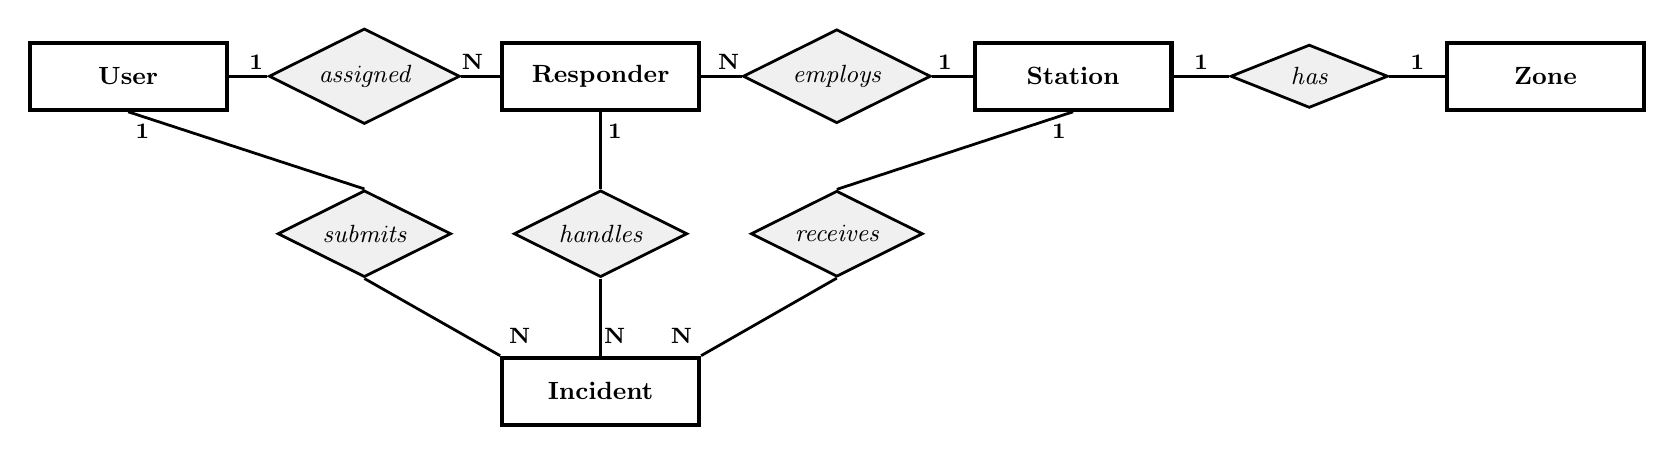
\begin{tikzpicture}[line width=1pt]

%% ── Entities ───────────────────────────────────────────
\node[entity] (user)      at ( 0, 4)  {User};
\node[entity] (responder) at ( 6, 4)  {Responder};
\node[entity] (station)   at (12, 4)  {Station};
\node[entity] (zone)      at (18, 4)  {Zone};
\node[entity] (incident)  at ( 6, 0)  {Incident};

%% ── Relationship diamonds ──────────────────────────────
\node[relship] (assigned) at ( 3, 4)  {assigned};   % User – Responder
\node[relship] (employs)  at ( 9, 4)  {employs};    % Station – Responder
\node[relship] (has)      at (15, 4)  {has};         % Station – Zone
\node[relship] (submits)  at ( 3, 2)  {submits};    % User – Incident
\node[relship] (handles)  at ( 6, 2)  {handles};    % Responder – Incident
\node[relship] (receives) at ( 9, 2)  {receives};   % Station – Incident

%% ── Connections ────────────────────────────────────────
% User –– assigned –– Responder  (1:N)
\draw (user.east)      -- (assigned.west);
\draw (assigned.east)  -- (responder.west);
\node[card] at ($(user.east)     +(0.35, 0.18)$) {1};
\node[card] at ($(responder.west)+(-0.35, 0.18)$) {N};

% Responder –– employs –– Station  (N:1)
\draw (responder.east) -- (employs.west);
\draw (employs.east)   -- (station.west);
\node[card] at ($(responder.east)+(0.35, 0.18)$)  {N};
\node[card] at ($(station.west) +(-0.35, 0.18)$)  {1};

% Station –– has –– Zone  (1:1)
\draw (station.east)  -- (has.west);
\draw (has.east)      -- (zone.west);
\node[card] at ($(station.east)+(0.35, 0.18)$)    {1};
\node[card] at ($(zone.west)   +(-0.35, 0.18)$)   {1};

% User –– submits –– Incident  (1:N)
\draw (user.south)     -- (submits.north);
\draw (submits.south)  -- (incident.north west);
\node[card] at ($(user.south)          +(0.18,-0.25)$) {1};
\node[card] at ($(incident.north west) +(0.25, 0.25)$) {N};

% Responder –– handles –– Incident  (1:N)
\draw (responder.south) -- (handles.north);
\draw (handles.south)   -- (incident.north);
\node[card] at ($(responder.south)+(0.18,-0.25)$) {1};
\node[card] at ($(incident.north) +(0.18, 0.25)$) {N};

% Station –– receives –– Incident  (1:N)
\draw (station.south)   -- (receives.north);
\draw (receives.south)  -- (incident.north east);
\node[card] at ($(station.south)       +(-0.18,-0.25)$) {1};
\node[card] at ($(incident.north east) +(-0.25, 0.25)$) {N};

\end{tikzpicture}
\end{document}
